\pagebreak\section{April 15, 2021}

We'll continue the discussion of Fourier series today -- last time, we defined the Fourier coefficients 
\[
    \hat{f}(n) = \frac{1}{2\pi} \int_{-\pi}^{\pi} f(t) e^{-int} dt
\]
for any function $f \in L^2([-\pi, \pi])$, which we can think of as the $L^2$ inner product of $f$ with $e^{-int}$ up to a constant. Defining the $N$th partial sums
\[
    S_Nf(x) = \sum_{n=-N}^N \hat{f}(n) e^{inx},
\]
we wanted to know whether $S_Nf$ always converges to $f$ in $L^2$ -- that is, whether for all $f \in L^2([-\pi, \pi])$ we have $\lim_{N \to \infty} ||f - S_N f||_2 = 0$.

Based on our discussion of Hilbert spaces, this question is equivalent to asking whether a function $f \in L^2([-\pi, \pi])$ with all Fourier coefficients zero must be the zero function (since we're trying to ask whether $\left\{\frac{1}{\sqrt{2\pi}} e^{inx}\right\}_{n \in \ZZ}$ is a maximal orthonormal subset). Our main step last time was to define the Cesaro-Fourier mean 
\[
    \sigma_N f(x) = \frac{1}{N+1} \sum_{k=0}^N S_k f(x),
\]
hoping that means of sequences converge better than the sequences themselves. Our goal is then to show that $||\sigma_N f - f||_2 \to 0$ as $N \to \infty$, and that will give us the desired convergence result for Fourier series.

We'll first rewrite the partial Fourier sums slightly differently, much like how we previously used the Dirichlet kernel:

\begin{proposition}
For all $f \in L^2([-\pi, \pi])$, we have 
\[
    \sigma_N f(x) = \int_{-\pi}^\pi K_N(x-t) f(t) dt, \quad K_N(x) = \begin{cases} \frac{N+1}{2\pi} & x = 0 \\ \frac{1}{2\pi(N+1)} \left(\frac{\sin\left(\frac{N+1}{2} x\right)}{\sin \frac{x}{2}}\right)^2 & \text{otherwise}. \end{cases}
\]
The function $K_N(x)$ is called the \vocab{Fej\'er kernel}, and it has the following properties: \textbf{(1)} $K_N(x) \ge 0$ and $K_N(x) = K_N(-x)$ for all $x$, \textbf{(2)} $K_N$ is periodic with period $2\pi$, \textbf{(3)} $\int_{-\infty}^{\infty} K_N(t) dt = 1$, and \textbf{(4)} for any $\delta \in (0, \pi)$ and for all $\delta \le |x| \le \pi$, we have $|K_N(x)| \le \frac{1}{2\pi(N+1) \sin^2\frac{\delta}{2}}$.
\end{proposition}

The idea is that the Fej\'er kernel grows more and more concentrated at the origin as $N \to \infty$, but the area of the curve is always $1$ (like the physics Dirac delta function) -- here's a picture for $N = 8$:

\centerline{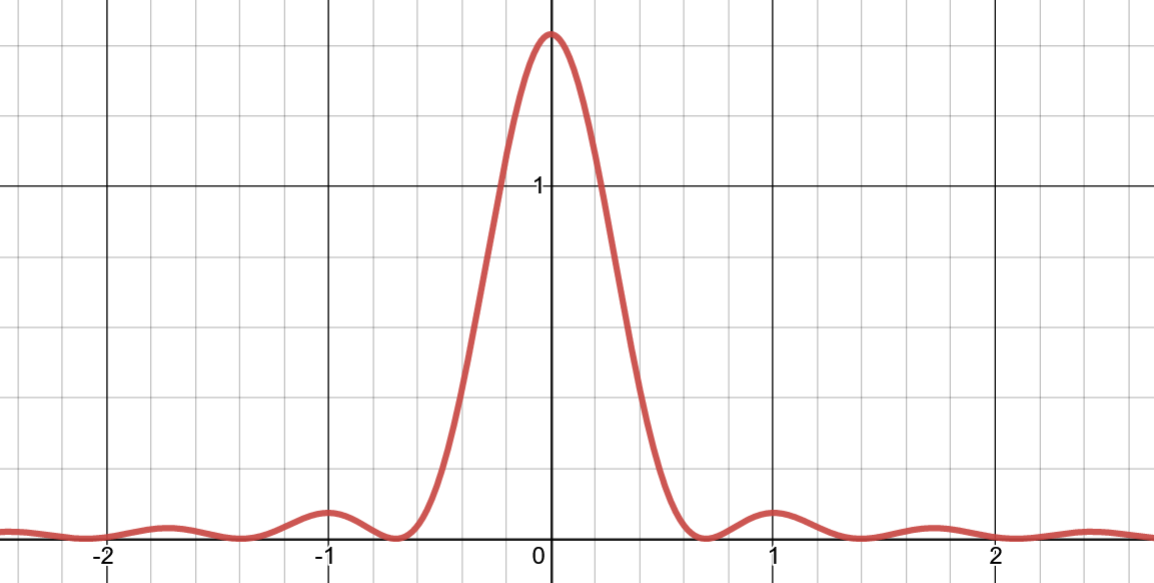
\includegraphics[width=8cm]{pictures/fejer.PNG}}

The reason we might believe that these Cesaro means converge to $f$ is that 
\[
    \sigma_N f(x) = \int_{-\pi}^\pi K_N(x-t) f(t) dt,
\]
and $K_N$ is very sharply peaked around $t = x$, so as $N$ gets larger and larger, the main contribution to the integral comes from $f(x) \approx f(t)$ if $f$ is well-behaved enough. So then we end up with 
\[
    \approx f(x) \int_{-\pi}^{\pi} K_N(x-t) dt = f(x) \cdot 1,
\]
since $k_N$ evaluates to the same over any interval of length $2\pi$ by periodicity. So that's a heuristic motivation for working with the Cesaro means here! (Some of these properties also applied when we did a similar procedure with our partial sums $S_Nf(x)$, but the \textbf{Dirichlet kernel is not nonnegative} -- that difference actually makes a big difference in the final proof.)

\begin{proof}
Recall that 
\[
    S_kf(x) = \int_{-\pi}^{\pi} D_k(x-t) f(t) dt
\]
for the Dirichlet kernel 
\[
    D_k(t) = \begin{cases} \frac{2N+1}{2\pi} & t = 0 \\ \frac{1}{2\pi} \frac{\sin\left(\left(N + \frac{1}{2}\right)t\right)}{\sin \frac{t}{2}} & \text{otherwise}. \end{cases}
\]
We can use this fact to find that 
\[
    \sigma_Nf(x) = \frac{1}{N+1} \sum_{k=0}^N S_kf(x) = \int_{-\pi}^{\pi} \frac{1}{N+1} \sum_{k=0}^N D_k(x-t) f(t) dt,
\]
and thus we know that the desired kernel is
\[
    K_N(x-t) = \frac{1}{N+1}\sum_{k=0}^N D_k(x-t).
\]
We can now substitute in our expression for $D_k$, using the variable $x$ instead of $x-t$. The case $x = 0$ can be done easily (we just have constants), and for all other $x$ we can slightly rewrite our expression as
\[
    K_N(x) = \frac{1}{2\pi(N+1)} \frac{1}{2\left(\sin \frac{x}{2}\right)^2} \sum_{k=0}^N 2\sin \frac{x}{2} \sin \left(\left(k + \frac12\right)x\right).
\]
By the trig product-to-sum identity, this simplifies to 
\[
    =  \frac{1}{2\pi(N+1)} \frac{1}{2\left(\sin \frac{x}{2}\right)^2} \sum_{k=0}^N \cos (kx) - \cos \left((k+1)x\right),
\]
and this is a telescoping sum which simplifies to 
\[
    = \frac{1}{2\pi(N+1)} \frac{1}{2\left(\sin \frac{x}{2}\right)^2} \left(1 - \cos((N+1)x)\right).
\]
We can now use another trig formula $\frac{1 - \cos x}{2} = \cos^2\left(\frac{x}{2}\right)$ to get 
\[
    =  \frac{1}{2\pi(N+1)} \frac{1}{\left(\sin \frac{x}{2}\right)^2} \sin^2\left(\frac{N+1}{2}x\right),
\]
which is indeed the expression for our Fej\'er kernel.

We can now verify the properties of the Fej\'er kernel directly: \textbf{(1)} is true because we have a manifestly positive expression and $\sin^2(cx)$ is even, and \textbf{(2)} is true because $\sin^2$ is also periodic with half the period of the corresponding $\sin$. For \textbf{(3)}, notice that 
\[
    \int_{-\pi}^\pi D_k(t) dt = \int_{-\pi}^\pi \sum_{n=-k}^k e^{int} dt,
\]
and the integral of $e^{int}$ is zero unless $n = 0$ (by $2\pi$-periodicity), so we just pick up the $n = 0$ term and get $1$. Since $\sigma_N$ is the average of the $D_k$s, the integral of $\sigma_N$ is also the average of the average of the $D_k$s, which will also be $1$.  

Finally, for \textbf{(4)}, notice that $\sin^2\frac{x}{2}$ is an even function which is increasing on $[0, \pi]$. So if we pick some $\delta \in (0, \pi)$, we can say that 
\[
    \delta \le |x| \le \pi \implies \sin^2\frac{x}{2} \ge \sin^2\frac{\delta}{2},
\]
so we indeed get the expected
\[
    K_N(x) = |K_N(x)| \le \frac{1}{2\pi(N+1) \sin^2\frac{\delta}{2}} \sin^2 \left(\frac{N+1}{2} x\right) \le \frac{1}{2\pi(N+1) \sin^2\frac{\delta}{2}}.
\]
\end{proof}

Now, we can prove convergence of the Cesaro means $\sigma_N f$ to $f$ by first doing it for continuous functions -- we showed that the continuous functions with endpoints $0$ are dense in $L^2$ (so we can show convergence appropriately), and continuous functions with endpoints both $0$ can indeed be treated as $2\pi$-periodic. So the subspace of $2\pi$-periodic continuous functions is dense in $L^2$, and we'll consider this dense subset first because it's where the heuristic argument we made above applies rigorously.

\begin{theorem}[Fej\'er]
Let $f \in C([-\pi, \pi])$ be $2\pi$-periodic (so $f(-\pi) = f(\pi)$). Then $\sigma_N f \to f$ uniformly on $[-\pi, \pi]$.
\end{theorem}

In other words, we have an even stronger result than $L^2$ convergence, now that we're limiting ourselves to continuous functions and have the stronger uniform norm. But this does \textbf{not} imply that the Fourier series of $f$ converges pointwise to $f$ -- there are indeed Fourier series representations of continuous functions that diverge at a point. Instead, it's the Cesaro mean and the Fej\'er kernel that help us out here!

\begin{proof}
First, we extend $f$ to all of $\RR$ by periodicity (defining it so that $f(x + 2\pi) = f(x)$ for all $x \in \RR$). Our function is then an element of $C(\RR)$ (still continuous), and it is $2\pi$-periodic, so it is uniformly continuous and bounded on all of $\RR$ (that is, $||f||_{\infty} = \sup_{x \in [-\pi, \pi]} f(x) < \infty$). 

We wish to show that $\sigma_N f$ converge uniformly on $f$, which means that for all $\eps > 0$ we need to find an $M$ so that for all $n \ge M$, we have $|\sigma_N f(x) - f(x)| < \eps$ for all $x$. Indeed, for any $\eps > 0$, by uniform continuity of $f$, there exists some $\delta > 0$ so that for all $|y-z| < \delta$, we have $|f(y) - f(z)| < \frac{\eps}{2}$. So now we can choose $M \in \NN$ so that for all $N \ge M$, we have
\[
    \frac{2||f||_{\infty}}{(N+1) \sin^2\frac{\delta}{2}} < \frac{\eps}{2}.
\]
(we can do this because the left-hand side converges to $0$ as $N \to \infty$). Now because $f$ and $K_N$ are $2\pi$-periodic, we can write the Cesaro mean as 
\[
    \sigma_N f(x) = \int_{-\pi}^{\pi} K_N(x-t) f(t) dt = \int_{x-\pi}^{x+\pi} K_N(\tau) f(x-\tau) d\tau
\]
by a change of variables (which is allowed because we're doing integrals over continuous functions, and thus we can use the Riemann integral), and now we have the product of $2\pi$-periodic functions, so the integral of that is the same over any interval of length $2\pi$: switching back to $t$ from $\tau$,
\[
    = \int_{-\pi}^{\pi} K_N(t) f(x-t) dt.
\]
We can now say that for all $N \ge M$ and for all $x \in [\pi, \pi]$, we have
\[
    |\sigma_N f(x) - f(x)| = \left|\int_{-\pi}^{\pi} K_N(t) f(x-t) dt - \int_{-\pi}^{\pi} K_N(t) f(x) dt\right|
\]
where we've added in a $\int_{-\pi}^{\pi} K_N(t) dt$ integral to the $f(x)$ term, which is okay because $f(x)$ doesn't talk to the $t$-integral. Combining the integrals by linearity gives us 
\[
    = \left|\int_{-\pi}^{\pi} K_N(t) \left(f(x-t) - f(x)\right) dt\right|.
\]
We'll use the triangle inequality and then split this integral into two parts now:
\[
    \le \int_{-\pi}^{\pi} \left| K_N(t) \left(f(x-t) - f(x)\right) \right| dt = \int_{|t| \le \delta} K_N(t) \left|f(x-t) - f(x)\right| dt + \int_{\delta \le |t| \le \pi} K_N(t) \left|f(x-t) - f(x)\right| dt
\]
(also using the fact that $K_N$ is always nonnegative). And now we can use our bounds above to simplify this: for the first term, we know that $|(x-t) - x| < \delta$ over the bounds of integration, so $|f(x-t) - f(x)| < \frac{\eps}{2}$. And for the second term, we know that $|f(x-t) - f(x)| < 2||f||_{\infty}$ because both $f(x-t)$ and $f(x)$ have magnitude at most $||f||_{\infty}$ for a continuous function, and when $|t| > \delta$ we can use condition \textbf{(4)} of the Fej\'er kernel. Putting this all together, we find the inequality
\[
    < \frac{\eps}{2}\int_{|t| \le \delta} K_N(t) dt + \frac{2||f||_\infty}{2\pi(N+1) \sin^2\frac{\delta}{2}} \int_{\delta \le |t| \le \pi} K_N(t) dt.
\]
We can now bound both integrals here by the integral over the entire region to get 
\[
    \le \frac{\eps}{2} + \frac{2||f||_{\infty}}{(N+1) \sin^2\frac{\delta}{2}} < \frac{\eps}{2} + \frac{\eps}{2} = \eps
\]
by our choice of $N$. So we've indeed shown uniform convergence -- $\sigma_N f$ is eventually close enough to $f$ for large enough $N$ -- and we're done. 
\end{proof}

\begin{remark}
This same proof can be modified if instead of knowing that $K_n(x) \ge 0$ (which we know for the Fej\'er kernel), we have that
\[
    \sup_N \int_{-\pi}^{\pi} |K_N(x)| < \infty.
\]
Then we can show the same uniform convergence by modifying our proof above. But if we try to plug in our Dirichlet kernel here, the condition is not satisfied, since 
\[
    \int_{-\pi}^{\pi} |D_N(x)| dx \sim \log N.
\]
So having ``almost all of the properties'' isn't enough for us to get the analogous results for the Dirichlet kernel!
\end{remark}

Now that we've proven that the Cesaro means of a continuous function converge uniformly to that function, we want to show that the Cesaro means of an $L^2$ function converge to an $L^2$ function, which would show the condition on the Hilbert space that we want and show convergence of the Fourier series as well. We'll first need the following result:

\begin{proposition}\label{cesaroineq}
For all $f \in L^2([-\pi, \pi])$, we have $||\sigma_N f||_2 \le ||f||_2$.
\end{proposition}
\begin{proof}
We'll first do this for $2\pi$-periodic functions. First suppose that $f \in C([-\pi, \pi])$ is $2\pi$-periodic -- extend $f$ to all of $\RR$ as before, and then the Cesaro mean is $\sigma_Nf(x) = \int_{-\pi}^{\pi} f(x-t) K_N(t) dt$. Thus, we can write out
\[
    \boxed{||\sigma_Nf||_2^2} = \int_{-\pi}^{\pi} |\sigma_Nf(x)|^2 dx = \int_{-\pi}^\pi \int_{-\pi}^\pi \int_{-\pi}^\pi f(x-s) \overline{f(x-t)} K_N(s) K_N(t) ds dt dx.
\]
All of these functions are continuous, so we can change the order of integration by Fubini's theorem to get 
\[
    = \int_{-\pi}^\pi \int_{-\pi}^\pi K_N(s) K_N(t) \left[\int_{-\pi}^{\pi} f(x-s) \overline{f(x-t)} dx\right] ds dt.
\]
By Cauchy-Schwarz, this can be bounded by 
\[
    \le \int_{-\pi}^\pi \int_{-\pi}^\pi K_N(s) K_N(t) ||f(\cdot -s)||_2 ||f(\cdot-t)||_2 ds dt,
\]
where $f(\cdot-s)$ denotes the function that maps $x \mapsto f(x-s)$. And now we're integrating a periodic function $f(\cdot -s)$ over an interval of length $2\pi$, so we can replace that expression with $||f||_2$ (just shifting to another length $2\pi$ interval). Doing the same with $f(\cdot -t)$ gives us
\[
    = ||f||_2^2\int_{-\pi}^\pi \int_{-\pi}^\pi K_N(s) K_N(t)  ds dt = \boxed{||f||_2^2},
\]
because the integral of $K_N$ is $1$. This gives us the desired inequality for $2\pi$-periodic functions, and now to extend it to all functions in $L^2$, suppose we have some general $f \in L^2$. From exercises, we know that there exists a sequence $\{f_n\}_n$ of $2\pi$-periodic continuous functions that converge to $f$ in $L^2$, meaning that $||f_n - f||_2 \to 0$. So from the definition of the Cesaro means, this means that $||\sigma_N f_n - \sigma_N f||_2 \to 0$ for any fixed $N$ and as $N \to \infty$, leading us to 
\[
    ||\sigma_N f||_2 = \lim_{n \to \infty} ||\sigma_N f_n||_2 \le \lim_{n \to \infty} ||f_n||_2
\]
(using the $2\pi$-periodic case), and this last result is $||f||_2$ because $f_n$ converges to $f$ in $L^2$.
\end{proof}

So now we're almost done, and combining the two results above will give us what we want:

\begin{theorem}
For all $f \in L^2$, $||\sigma_N f - f||_2 \to 0$ as $N \to \infty$. Therefore, if $\hat{f}(n) = 0$ for all $n$, then $f = 0$ (since $\sigma_N f = 0$ for all $N$).
\end{theorem}
\begin{proof}
(We only need to prove the result in the first sentence -- the second follows directly as stated.) Let $f \in L^2([-\pi, \pi])$, and let $\eps > 0$. By density of the $2\pi$-periodic continuous functions, there exists some $2\pi$-periodic $g \in C([-\pi, \pi])$ so that $||f-g||_2 < \frac{\eps}{3}$. Because $\sigma_N g \to g$ uniformly on $[-\pi, \pi]$, there exists some $M$ so that for all $N \ge M$ and for all $x \in [-\pi, \pi]$, we have $|\sigma_Ng(x) - g(x)| < \frac{\eps}{3\sqrt{2\pi}}$.  

Now for all $N \ge M$, the triangle inequality tells us that
\[
    ||\sigma_Nf - f||_2 \le ||\sigma_N f - \sigma_N g||_2 + ||\sigma_N g - g||_2 + ||g - f||_2.
\]
The first term is $||\sigma_N(f-g)||_2$ (we can check this from the definition), and by \cref{cesaroineq}, that is less than $||f-g||_2 < \frac{\eps}{3}$. Meanwhile, the last term is also bounded by $\frac{\eps}{3}$, and the middle term is $\left(\int_{-\pi}^{\pi} |\sigma_N g(x) - g(x) |^2 dx \right)^{1/2} < \left(2\pi \cdot\left(\frac{\eps}{3\sqrt{2\pi}}\right)^2\right)^{1/2} = \frac{\eps}{3}$. So putting this all back into our expression gives us
\[
     ||\sigma_Nf - f||_2 < \frac{\eps}{3} + \frac{\eps}{3} + \frac{\eps}{3} = \eps,
\]
completing the proof.
\end{proof}

So we've now seen a concrete application of the general machinery we've built up for Hilbert spaces! In summary, we've shown that the normalized exponentials form a maximal orthonormal set, so that the partial Fourier sums of $f$ converge to $f$ in $L^2$. But as previous mentioned, we don't have pointwise convergence everywhere -- instead, we can only say that there is a \textbf{subsequence} that converges to $f$ pointwise. And in fact, \textbf{Carleson's theorem }is a deep result in analysis that tells us that for all $f \in L^2$, $S_Nf(x) \to f(x)$ \textbf{almost everywhere}.

We can also ask questions about the convergence of Fourier series in other $L^p$ spaces, since all of the definitions also make sense there. It is known additionally that for all $1 < p < \infty$, we always have $||S_N f - f||_p \to 0$, and that this is false for $p = 1, \infty$. But deeper harmonic analysis is needed to prove statements like this, and in particular we would need to learn how to work with \textbf{singular integral operators}.

In this class, though, this is as far as we'll go with Fourier series, and next time, we'll move on to the topic of \textbf{minimizers over closed convex sets} and (as a consequence) how to identify the dual of a Hilbert space with the Hilbert space itself in a canonical way. 